\documentclass[12pt]{article}
\usepackage[utf8]{inputenc}
\usepackage{amsmath}
\usepackage{amssymb}
\usepackage{mathtools}
\usepackage{amsfonts}
\usepackage{lastpage}
\usepackage{tikz}
\usepackage{pdfpages}
\usepackage{gauss}
\usepackage{fancyvrb}
\usepackage{fancyhdr}
\usepackage{graphicx}
\pagestyle{fancy}
\fancyfoot[C]{\footnotesize Page \thepage\ of 3}
\DeclareGraphicsExtensions{.pdf,.png,.jpg}
\title{Elementær Talteori}
\author{Nikolaj Dybdahl Rathcke}
\chead{Nikolaj Dybdahl Rathcke (rfq695)}

\begin{document}
Vi ser at det er det karakteristiske polynomium
$$\lambda^2-2\lambda+3=0$$
Med rødderne\\
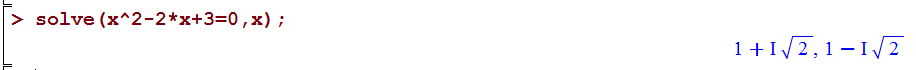
\includegraphics[width=\textwidth]{2}\\
hvor begge rødder er komplekse og har multiplicitet 1, så $\lambda_1=1+I\sqrt{2}$ og $\lambda_2=1-I\sqrt{2}$.\\
Vi kan så finde basis løsningerne ved brug af Maple.
\begin{align*}
x(1+I\sqrt{2})&=[\lambda_1^1,\lambda_1^2,\lambda_1^3,\lambda_1^4,...] \\
&=[1+I\sqrt{2},-1+2I\sqrt{2},-5+I\sqrt{2},-7-4I\sqrt{2},...] \\
x(1-I\sqrt{2})&=[\lambda_2^1,\lambda_2^2,\lambda_2^3,\lambda_2^4,...] \\
&=[1-I\sqrt{2},-1-2I\sqrt{2},-5-I\sqrt{2},-7+4I\sqrt{2},...] \\
\end{align*}
Og igen er basis løsningerne altså
\begin{align*}
x_1&=[1+I\sqrt{2},-1+2I\sqrt{2},-5+I\sqrt{2},-7-4I\sqrt{2},...] \\
x_2&=[1-I\sqrt{2},-1-2I\sqrt{2},-5-I\sqrt{2},-7+4I\sqrt{2},...] 
\end{align*}

\end{document}
